\documentclass[main.tex]{subfiles}

\begin{document}

\section{Priority CP}
\usingnamespace{pcp}

\begin{figure}[t]
  \centering
  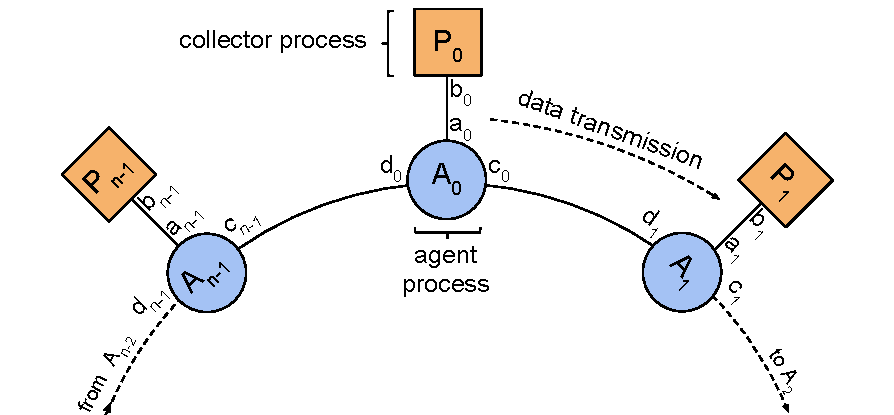
\includegraphics[width=0.8\columnwidth]{scheduler}
  \vspace{-4mm}
  \caption{Cyclic Scheduler from \cite{dardha2018}}
  \label{fig:scheduler}
  \vspace{-4mm}
  \end{figure}

\subsection{Syntax}

In this section we present an updated version of Priority CP~\cite{dardha2018}, which is Wadler's Classical Processes~\cite{wadler2012} with \emph{priorities}.

% Wen: Do we have to mention this? I'm assuming this was mentioned in~\cite{dardha2018}?
% "Some details of the calculus are inspired by Carbone \emph{et al.}~\cite{carbone2016} and Caires and P\'{e}rez~\cite{caires2017}."

\paragraph*{Priorities, types, and environments}
Types are based on classical linear logic formulas, and are annotated with priorities $\cs{o}\in\mathbb{N}$.

The types $\ty{\tytens[\cs{o}]{A}{B}}$ and $\ty{\typarr[\cs{o}]{A}{B}}$ type the endpoints of a channel over which we send or receive a channel of type $\ty{A}$, and then proceed as $\ty{B}$.
The types $\ty{\tyone[\cs{o}]}$ and $\ty{\tybot[\cs{o}]}$ type the endpoints of a channel over which we send or receive a ping, and then close the channel. These act as the units for $\ty{\tytens[\cs{o}]{A}{B}}$ and $\ty{\typarr[\cs{o}]{A}{B}}$.

The types $\ty{\typlus[\cs{o}]{A}{B}}$ and $\ty{\tywith[\cs{o}]{A}{B}}$ type the endpoints of a channel over which we can make or offer a choice between two options $\ty{A}$ or $\ty{B}$.
The types $\ty{\tynil[\cs{o}]}$ and $\ty{\tytop[\cs{o}]}$ type the endpoints of a channel over which we can make offer a choice between \emph{no options}. These act as the units for $\ty{\typlus[\cs{o}]{A}{B}}$ and $\ty{\tywith[\cs{o}]{A}{B}}$.
\[
\begin{array}{lcl}
  \ty{A}, \ty{B}, \ty{C}
  & \coloneqq & \ty{\tytens[\cs{o}]{A}{B}}
    \sep        \ty{\typarr[\cs{o}]{A}{B}}
    \sep        \ty{\tyone[\cs{o}]}
    \sep        \ty{\tybot[\cs{o}]}
    \sep        \ty{\typlus[\cs{o}]{A}{B}}
    \sep        \ty{\tywith[\cs{o}]{A}{B}}
    \sep        \ty{\tynil[\cs{o}]}
    \sep        \ty{\tytop[\cs{o}]}
\end{array}
\]
A typing context $\ty\Gamma$ is a partial function associating channel names to types.
\[
\begin{array}{lcl}
  \ty{\Gamma}, \ty{\Delta}
  & \coloneqq & \ty{\emptyenv}
    \sep        \ty{\Gamma}, \tmty{x}{A}
\end{array}
\]
Duality on types is an involutive function which preserves the priorities of types.
\[
\begin{array}{lcl}
  \ty{\co{(\tyone[\cs{o}])}} & = & \ty{\tybot[\cs{o}]} \\
  \ty{\co{(\tybot[\cs{o}])}} & = & \ty{\tyone[\cs{o}]} \\
  \ty{\co{(\tynil[\cs{o}])}} & = & \ty{\tytop[\cs{o}]} \\
  \ty{\co{(\tytop[\cs{o}])}} & = & \ty{\tynil[\cs{o}]}
\end{array}
\qquad
\begin{array}{lcl}
  \ty{\co{(\tytens[\cs{o}]{A}{B})}} & = & \ty{\typarr[\cs{o}]{\co{A}}{\co{B}}} \\
  \ty{\co{(\typarr[\cs{o}]{A}{B})}} & = & \ty{\tytens[\cs{o}]{\co{A}}{\co{B}}} \\
  \ty{\co{(\typlus[\cs{o}]{A}{B})}} & = & \ty{\tywith[\cs{o}]{\co{A}}{\co{B}}} \\
  \ty{\co{(\tywith[\cs{o}]{A}{B})}} & = & \ty{\typlus[\cs{o}]{\co{A}}{\co{B}}}
\end{array}
\]
The function $\pr(\cdot)$ returns the priority of a type. The function $\minpr(\cdot)$ returns the \emph{minimum} priority of all types a typing context.
\[
\begin{array}{lclclcl}
  \pr(\ty{\tyone[\cs{o}]})        & = & \cs{o}  \\
  \pr(\ty{\tybot[\cs{o}]})        & = & \cs{o}  \\
  \pr(\ty{\tynil[\cs{o}]})        & = & \cs{o}  \\
  \pr(\ty{\tytop[\cs{o}]})        & = & \cs{o}  \\
  \\
  \minpr(\ty{\emptyenv})          & = & \varnothing
\end{array}
\qquad
\begin{array}{lclclcl}
  \pr(\ty{\tytens[\cs{o}]{A}{B}}) & = & \cs{o}  \\
  \pr(\ty{\typarr[\cs{o}]{A}{B}}) & = & \cs{o}  \\
  \pr(\ty{\typlus[\cs{o}]{A}{B}}) & = & \cs{o}  \\
  \pr(\ty{\tywith[\cs{o}]{A}{B}}) & = & \cs{o}  \\
  \\
  \minpr(\ty{\Gamma},\tmty{x}{A}) & = & \minpr(\ty{\Gamma})\sqcap\minpr(\ty{A})
\end{array}
\]

\paragraph*{Terms}
\[
\begin{array}[t]{lcl}
  \tm{P}, \tm{Q}
  & \coloneqq & \tm{\link{x}{y}}
         \sep   \tm{\res{x}{x'}{P}}
         \sep   \tm{(\ppar{P}{Q})}
         \sep   \tm{\halt}
  \\   & \sep & \tm{\send{x}{y}{P}}
         \sep   \tm{\close{x}{P}}
         \sep   \tm{\recv{x}{y}{P}}
         \sep   \tm{\wait{x}{P}}
  \\   & \sep & \tm{\inl{x}{P}}
         \sep   \tm{\inr{x}{P}}
         \sep   \tm{\offer{x}{P}{Q}}
         \sep   \tm{\absurd{x}}
\end{array}
\]

\paragraph*{Syntactic Sugar}
We define \emph{unbound} send:
\[
  \tm{\usend{x}{y}{P}}\elabarrow\tm{\send{x}{z}{(\ppar{\link{y}{z}}{P})}}
\]

\subsection{Typing}
See \cref{fig:pcp-typing}.
\begin{figure}[H]
  \begin{mdframed}
    \begin{mathpar}
      \inferrule*[lab=T-Link]{
      }{\seq{\link[\ty{A}]{x}{y}}{\tmty{x}{A},\tmty{y}{\co{A}}}}
      
      \inferrule*[lab=T-Res]{
        \seq{P}{\ty{\Gamma},\tmty{x}{A},\tmty{y}{\co{A}}}
      }{\seq{\res{x}{y}{P}}{\ty{\Gamma}}}
      \\
      \inferrule*[lab=T-Par]{
        \seq{P}{\ty{\Gamma}}
        \\
        \seq{Q}{\ty{\Delta}}
      }{\seq{\ppar{P}{Q}}{\ty{\Gamma},\ty{\Delta}}}
      
      \inferrule*[lab=T-Halt]{
      }{\seq{\halt}{\emptyenv}}
      \\
      \inferrule*[lab=T-Send]{
        \seq{P}{\ty{\Gamma},\tmty{y}{A},\tmty{x}{B}}
        \\
        \cs{o}<\minpr(\ty{\Gamma},\ty{A},\ty{B})
      }{\seq{\send{x}{y}{P}}{\ty{\Gamma},\tmty{x}{\tytens[\cs{o}]{A}{B}}}}
      
      \inferrule*[lab=T-Close]{
        \seq{P}{\ty{\Gamma}}
        \\
        \cs{o}<\minpr(\ty{\Gamma})
      }{\seq{\close{x}{P}}{\ty{\Gamma},\tmty{x}{\tyone[\cs{o}]}}}
      \\
      \inferrule*[lab=T-Recv]{
        \seq{P}{\ty{\Gamma},\tmty{y}{A},\tmty{x}{B}}
        \\
        \cs{o}<\minpr(\ty{\Gamma},\ty{A},\ty{B})
      }{\seq{\recv{x}{y}{P}}{\ty{\Gamma},\tmty{x}{\typarr[\cs{o}]{A}{B}}}}
      
      \inferrule*[lab=T-Wait]{
        \seq{P}{\ty{\Gamma}}
        \\
        \cs{o}<\minpr(\ty{\Gamma})
      }{\seq{\wait{x}{P}}{\ty{\Gamma},\tmty{x}{\tybot[\cs{o}]}}}
      \\
      \inferrule*[lab=T-Select-Inl]{
        \seq{P}{\ty{\Gamma},\tmty{x}{A}}
        \\
        \cs{o}<\minpr(\ty{\Gamma},\ty{A},\ty{B})
        \\
        \pr(\ty{A})=\pr(\ty{B})
      }{\seq{\inl{x}{P}}{\ty{\Gamma},\tmty{x}{\typlus[\cs{o}]{A}{B}}}}
      
      \inferrule*[lab=T-Select-Inr]{
        \seq{P}{\ty{\Gamma},\tmty{x}{B}}
        \\
        \cs{o}<\minpr(\ty{\Gamma},\ty{A},\ty{B})
        \\
        \pr(\ty{A})=\pr(\ty{B})
      }{\seq{\inr{x}{P}}{\ty{\Gamma},\tmty{x}{\typlus[\cs{o}]{A}{B}}}}
      
      \inferrule*[lab=T-Offer]{
        \seq{P}{\ty{\Gamma},\tmty{x}{A}}
        \\
        \seq{Q}{\ty{\Gamma},\tmty{x}{B}}
        \\
        \cs{o}<\minpr(\ty{\Gamma},\ty{A},\ty{B})
      }{\seq{\offer{x}{P}{Q}}{\ty{\Gamma},\tmty{x}{\tywith[\cs{o}]{A}{B}}}}
      
      \inferrule*[lab=T-Offer-Absurd]{
        \cs{o}<\pr(\ty{\Gamma})
      }{\seq{\absurd{x}}{\ty{\Gamma},\tmty{x}{\tytop[\cs{o}]}}}
    \end{mathpar}
    \caption{Typing Rules for PCP.}
    \label{fig:pcp-typing}
  \end{mdframed}
\end{figure}
%%% Local Variables:
%%% TeX-master: "../priorities"
%%% End:


\subsection{Operational Semantics}
See \cref{fig:pcp-operational-semantics}.
\begin{figure}
  \begin{mdframed}
    \small
    \paragraph*{Structural congruence}
    \begin{mathpar}
      \begin{array}{llcl}
        \LabTirName{SC-LinkSwap}   & \tm{\link{x}{y}}
                                   & \equiv & \tm{\link{y}{x}}
        \\
        \LabTirName{SC-ResLink}    & \tm{\res{x}{y}{\link{x}{y}}}
                                   & \equiv & \tm{\halt}
        \\
        \LabTirName{SC-ResSwap}    & \tm{\res{x}{y}{P}}
                                   & \equiv & \tm{\res{y}{x}{P}}
        \\
        \LabTirName{SC-ResComm}    & \tm{\res{x}{y}{\res{z}{w}{P}}}
                                   & \equiv & \tm{\res{z}{w}{\res{x}{y}{P}}}
        \\
        \LabTirName{SC-ResExt}     & \tm{\res{x}{y}{(\ppar{P}{Q})}}
                                   & \equiv & \tm{\ppar{P}{\res{x}{y}{Q}}},
                                              \text{ if }{\tm{x},\tm{y}\notin\fv(\tm{P})}
        \\
        \LabTirName{SC-ParNil}     & \tm{\ppar{P}{\halt}}
                                   & \equiv & \tm{P}
        \\
        \LabTirName{SC-ParComm}    & \tm{\ppar{P}{Q}}
                                   & \equiv & \tm{\ppar{Q}{P}}
        \\
        \LabTirName{SC-ParAssoc}   & \tm{\ppar{P}{(\ppar{Q}{R})}}
                                   & \equiv & \tm{\ppar{(\ppar{P}{Q})}{R}}
      \end{array}
    \end{mathpar}
    
    \paragraph*{Reduction}
    \begin{mathpar}
      \begin{array}{llcl}
        \LabTirName{E-Link}    & \tm{\res{x}{y}{(\ppar{\link{w}{x}}{P})}}
                               & \red & \tm{\subst{P}{w}{x}}
        \\
        \LabTirName{E-Send}    & \tm{\res{x}{y}{(\ppar{\send{x}{z}{P}}{\recv{x}{w}{Q}})}}
                               & \red & \tm{\res{x}{y}{\res{z}{w}{(\ppar{P}{Q})}}}
        \\
        \LabTirName{E-Close}   & \tm{\res{x}{y}{(\ppar{\close{x}{P}}{\wait{y}{Q}})}}
                               & \red & \tm{\ppar{P}{Q}}
        \\
        \LabTirName{E-Select-Inl}
                               & \tm{\res{x}{y}{(\ppar{\inl{x}{P}}{\offer{x}{Q}{R}})}}
                               & \red & \tm{\res{x}{y}{(\ppar{P}{Q})}}
        \\
        \LabTirName{E-Select-Inr}
                               & \tm{\res{x}{y}{(\ppar{\inr{x}{P}}{\offer{x}{Q}{R}})}}
                               & \red & \tm{\res{x}{y}{(\ppar{P}{R})}}
      \end{array}
      \\
      \inferrule*[lab=E-LiftRes]{
        \tm{P}\red\tm{P'}
      }{\tm{\res{x}{y}{P}}\red\tm{\res{x}{y}{P'}}}
    
      \inferrule*[lab=E-LiftPar]{
        \tm{P}\red\tm{P'}
      }{\tm{\ppar{P}{Q}}\red\tm{\ppar{P'}{Q}}}
    
      \inferrule*[lab=E-LiftSC]{
        \tm{P}\equiv\tm{P'}
        \\
        \tm{P'}\red\tm{Q'}
        \\
        \tm{Q'}\equiv\tm{Q}
      }{\tm{P}\red\tm{Q}}
    \end{mathpar}
    \caption{Operational Semantics for PCP.}
    \label{fig:pcp-operational-semantics}
  \end{mdframed}
\end{figure}
%%% Local Variables:
%%% TeX-master: "../priorities"
%%% End:


\subsection{Metatheory}

\begin{restatablelemma}{lempcpsubjectcongruence}[Subject Congruence, $\equiv$]
  \label{lem:pcp-subject-congruence}
  \hfill\\%newline before theorem statement
  If $\seq{P}{\ty{\Gamma}}$ and $\tm{P}\equiv\tm{Q}$,
  then $\seq{Q}{\ty{\Gamma}}$.
\end{restatablelemma}
\begin{proof}
  See~\cite{dardha2018}.
\end{proof}

\begin{restatabletheorem}{thmpcpsubjectreduction}[Subject Reduction, $\red$]
  \label{thm:pcp-subject-reduction}
  \hfill\\%newline before theorem statement
  If $\seq{P}{\ty{\Gamma}}$ and $\tm{P}\red\tm{Q}$, then $\seq{Q}{\ty{\Gamma}}$.
\end{restatabletheorem}
\begin{proof}
  See~\cite{dardha2018}.
\end{proof}

\begin{definition}[Actions]
  A~process acts on an endpoint $\tm{x}$ if it is in one of the following forms:
  \begin{multicols}{3}
    \begin{itemize}[noitemsep,topsep=0pt,parsep=0pt,partopsep=0pt]
    \item $\tm{\link{x}{y}}$ 
    \item $\tm{\link{y}{x}}$
    \item $\tm{\send{x}{y}{P}}$
    \item $\tm{\recv{x}{y}{P}}$
    \item $\tm{\close{x}{P}}$
    \item $\tm{\wait{x}{P}}$
    \item $\tm{\inl{x}{P}}$
    \item $\tm{\inr{x}{P}}$
    \item $\tm{\offer{x}{P}{Q}}$
    \item $\tm{\absurd{x}}$
    \end{itemize}
  \end{multicols}
  \noindent
  A~process is an action if it acts on on some endpoint $\tm{x}$.
\end{definition}

\begin{definition}[Canonical Forms]
  \label{def:pcp-canonical-forms}
  A~process $\tm{P}$ is in canonical form if it is in one of the following forms:
  \begin{itemize}[noitemsep,topsep=0pt,parsep=0pt,partopsep=0pt]
  \item
    $\tm{\halt}$
  \item
    $\tm{\res{x_1}{x'_1}{\dots\res{x_n}{x'_n}{(P_1 \parallel\dots\parallel P_m)}}}$
    where $m>0$ and each $\tm{P_j}$ is an action.
  \end{itemize}
\end{definition}

\begin{restatablelemma}{lempcpcanonicalforms}[Canonical Forms]
  \label{lem:pcp-canonical-forms}
  If $\seq{P}{\ty{\Gamma}}$, there exists some $\tm{Q}$ such that $\tm{P}\equiv\tm{Q}$ and $\tm{Q}$ is in canonical form.
\end{restatablelemma}
\begin{proof}
  If $\tm{P}=\tm{\halt}$, we are done. Otherwise, we move any $\nu$-binders to the top using \LabTirName{SC-ResExt}, and discard any superfluous occurrences of $\tm{\halt}$ using \LabTirName{SC-ParNil}.
\end{proof}

\begin{restatabletheorem}{thmpcpclosedprogress}[Closed Progress, $\red$]
  \label{thm:pcp-closed-progress}
  \hfill\\%newline before theorem statement
  If $\seq{P}{\emptyenv}$ and $\tm{P}$ is in canonical form, then either $\tm{P}=\tm{\halt}$ or there exists a $\tm{Q}$ such that $\tm{P}\red\tm{Q}$.
\end{restatabletheorem}
\begin{proof}
  Details in~\cref{prf:thm-pcp-closed-progress}.
\end{proof}

\end{document}

%%% Local Variables:
%%% TeX-master: "priorities"
%%% End:
